% ============================================================
% APPENDIX E -- Axiomatic Capability Realisation Model
% ============================================================

\label{app:crf}

\begin{ataglance}[The argument in outline]
This chapter has several moving parts, so it is worth setting out its shape before
any equations appear. Each section does one of the following six things.
\begin{enumerate}\setlength{\itemsep}{2pt}
\item \emph{Decide what ``realised'' means.} Realised potential is biomedical
potential $P$ scaled down by how far social enablement $S$ and structural freedom
$R$ fall short of full. The quantity of interest is that shortfall; it is zero only
when the context is perfect.
\item \emph{State the rules first (the baseline).} Six axioms fix what any
realisation measure must do, chief among them \emph{non-compensation}: no amount of
biomedical advantage can cancel complete social exclusion or complete structural
obstruction.
\item \emph{Fix the boundary (the junction with the world).} Two conditions pin the
model to reality: perfect context returns full potential, $H(P,1,1)=P$; total
exclusion returns none, $H(P,0,R)=H(P,S,0)=0$.
\item \emph{Derive the one admissible form.} Requiring constant contextual
elasticities singles out the geometric model $H=P\,S^{\alpha}R^{1-\alpha}$; a
substitution parameter $\rho<0$ gives the wider non-compensatory family.
\item \emph{Push it and read the gradients (the perturbation).} Marginal effects,
an exact capability-gap decomposition, and a budget-constrained policy gradient say
how realised potential moves when an intervention changes a domain.
\item \emph{Check it survives (the stability).} An equity-sensitive population
measure and a pre-specified head-to-head comparison decide whether the model holds
or must be narrowed.
\end{enumerate}
Two further pieces frame the policy use: an \emph{identification problem} that says why
a model is needed at all rather than reading capability off observed behaviour, and a
\emph{non-transportability} result that says why a policy ranking proven in one setting
need not hold in another. The realised score also feeds an eight-coordinate policy
evidence vector rather than a single cost-per-outcome threshold.
One convention about the equations. Every numbered equation below is one of three
things: a \emph{definition}, which introduces a symbol; a \emph{structural relation},
which states a property the model is required to have; or a \emph{consequence},
obtained from earlier equations. Consequences name which equations were used, so any
step can be checked without reconstructing it.
\end{ataglance}

\begin{ataglance}[How to read this appendix]
This is the formal core of the thesis and it builds one object in eight steps.
It starts with a problem rather than a formula: several different aggregation
rules fit the same data, so the data cannot choose between them
(\S\ref{sec:E-identification}). It fixes the objects and states six axioms
(\S\ref{sec:E-axioms}), notes that two rival ontologies satisfy different ones
(\S\ref{sec:E-ontologies}), and derives the family of functions that survive
(\S\ref{sec:E-family}). A characterisation theorem then shows exactly which
extra assumption picks out the primary form
(\S\ref{sec:E-characterisation}).

From that form four results follow, and they are the payload. The
cross-partials are positive, which is intersectionality written as
mathematics (\S\ref{sec:E-marginal}). Any gap between two people or groups
splits exactly into three named parts with no residual
(\S\ref{sec:E-gap}). A budget-constrained gradient says where the next unit of
money buys the most (\S\ref{sec:E-gradient}). And an equity-sensitive
population functional says how to add people up without pretending the
addition is value-free.

Two theorems bound the ambition. Policy rankings do not transport between
jurisdictions even when the clinical effect does
(\S\ref{sec:E-transport}), and the whole construction is falsifiable by
pre-specified tests (\S\ref{sec:E-falsification}).

Mrs~A and Mr~B are carried through with numbers so that each result can be
checked against a case rather than taken on trust.
\end{ataglance}

\section{Purpose and Status}
This chapter presents the central formal contribution of the thesis: an axiomatic
Capability Realisation Function (CRF) that turns the conceptual claim of health as
capability-in-context into a falsifiable mathematical model, together with an
integrated, equity-sensitive policy calculation built on it. Where the earlier
conceptual expression $(L\cdot Q)S-B$ was only a heuristic, the CRF derives realised
potential from stated axioms, proves its properties, supplies an exact
capability-gap decomposition and a budget-constrained policy gradient, and defines
the comparisons capable of rejecting it. The aggregation family is a new
specification within the $H_{\text{potential}}$ framework; its ingredients,
including constant-elasticity \citep{arrow_chenery_1961} and geometric means, are established mathematical
tools, and no priority claim is made for those tools themselves. The measurement
model of the preceding chapters supplies the outcome-independent domain scores
against which the CRF is tested head-to-head.

The reason a formal treatment is needed at all is that the obvious empirical
strategy, fitting several candidate rules and keeping the best, does not work
here. The next section says why.

\section{The Identification Problem}
\label{sec:E-identification}
The model exists to solve a problem that cross-sectional data cannot solve on their
own. Let $\mathcal{C}_i$ be the set of health-related functionings genuinely open to
person $i$, and let $F_i=\chi_i(\mathcal{C}_i)$ be the functioning actually observed,
where $\chi_i$ encodes that person's choices and preferences. Observed functioning
does not identify the opportunity set \citep{sen_1993}:
\begin{equation}
F_i=\chi_i(\mathcal{C}_i), \qquad F_i=F_j \;\nRightarrow\; \mathcal{C}_i=\mathcal{C}_j .
\label{eq:identification}
\end{equation}
Two people with identical observed activity may hold very different capability sets
if one acted without constraint while the other reached the same level through great
effort under severe structural bottlenecks. No amount of cross-sectional observation
separates the two without an explicit model of biological reserve, enabling
conditions and structural constraints. The Capability Realisation Function is that
model: it reconstructs realised capability from $P$, $S$ and $R$ rather than reading
it off achieved functioning.
\begin{reading}[Why a model is needed at all]
If we measure only what people currently do, we cannot tell a free choice from a
blocked one: the same score can mean ``well and choosing to rest'' or ``able but
prevented''. This chapter's function is the minimal apparatus that lets those two be
different, by carrying capacity and context as separate inputs.

Carrying them separately requires saying precisely what each is, on what scale
it is measured, and what any rule combining them must respect.
\end{reading}

\section{Objects, Scale, and Axioms}
\label{sec:E-axioms}
For person $i$, let $P_i=L_iQ_i\geq0$ be biomedical potential measured in
quality-adjusted life-years, $S_i\in[0,1]$ social enablement, and
$B_i\in[0,1]$ structural burden. Define structural freedom $R_i=1-B_i$.
The realised potential $H(P,S,R)$ is required to satisfy:
\begin{enumerate}
 \item \textbf{Dimensional coherence:} $H$ has the units of $P$.
 \item \textbf{Normalisation:} $H(P,1,1)=P$.
 \item \textbf{Monotonicity:} $H$ is non-decreasing in $P,S,R$.
 \item \textbf{Bounded realisation:} $0\leq H(P,S,R)\leq P$.
 \item \textbf{Essential enablement:} for $P>0$, $H(P,0,R)=H(P,S,0)=0$.
 \item \textbf{Replication invariance:} changing the measurement units used
 to construct a normalised domain does not change the ordering of $H$.
\end{enumerate}
The fifth axiom encodes non-compensation: complete social exclusion or complete
structural obstruction cannot be cancelled by biomedical advantage.

\begin{notationtable}
$P=L\cdot Q$ & Biomedical potential & Disease-adjusted life expectancy $L$ scaled by a quality-of-life multiplier $Q$; the health capacity a person has, in quality-adjusted life-years. \\
\addlinespace
$S\in[0,1]$ & Social enablement & The interpersonal and service resources that let capacity be used; $1$ is full enablement, $0$ complete exclusion. \\
\addlinespace
$B\in[0,1]$ & Structural burden & Structural and system constraints; $1$ is total obstruction. \\
\addlinespace
$R=1-B$ & Structural freedom & The room the structure leaves for capacity to be realised. \\
\addlinespace
$H(P,S,R)$ & Realised potential & How much of $P$ the context actually lets a person realise; the chapter's central object. \\
\addlinespace
$\alpha\in(0,1)$ & Social share & How much weight realisation places on social enablement relative to structural freedom. \\
\addlinespace
$\rho\leq0$ & Substitution parameter & How far a surplus in one enabler can stand in for a shortfall in the other; $\rho\to-\infty$ is no substitution at all. \\
\addlinespace
$\varepsilon\geq0$ & Inequality aversion & How strongly the population measure prioritises people with low realised potential. \\
\end{notationtable}

\section{Two Ontologies: Capacity-Ceiling and Relational}
\label{sec:E-ontologies}
Axiom~4 (bounded realisation) encodes a specific ontological choice, and it is worth
stating the alternative it rules out. Under the \emph{capacity-ceiling} ontology,
biological potential $P$ is the non-negotiable upper bound and context is a
conversion factor \citep{venkatapuram_2011,who_2015_ageing}:
\begin{equation}
H^{C}(P,S,R)=P\cdot M(S,R),\qquad 0\le M(S,R)\le 1 \;\Rightarrow\; 0\le H^{C}\le P .
\label{eq:ceiling}
\end{equation}
No degree of social support or structural optimisation lets a person exceed their
raw biological ceiling. Under the \emph{relational} ontology, capability is jointly
constituted by biology and environment, so assistive technology, institutional
modification or specialised support can raise effective capability above an
unassisted biological reading \citep{venkatapuram_2011,who_2015_ageing}:
\begin{equation}
H^{R}(P,S,R)=G(P,S,R),\qquad \text{with } H^{R}\le P \text{ not required.}
\label{eq:relational}
\end{equation}
The Capability Realisation Function developed here is the capacity-ceiling
operationalisation: it satisfies $H\le P$ by construction and is the conservative,
testable default. The relational extension, in which the conversion factor may exceed
one for a specific assistive mechanism, is a declared direction for future work;
adopting it would relax Axiom~4 and must be argued for a named mechanism rather than
assumed.
\begin{reading}[What the choice commits us to]
The capacity-ceiling model says context can only help a person use the health they
have, never manufacture more; it cannot represent a wheelchair that expands real
functioning beyond the unaided body. That is a deliberate, cautious commitment: it
keeps the metric bounded and interpretable, and it flags the relational case as a
separate claim to be made explicitly.
\end{reading}

\section{Capability Realisation Family}
\label{sec:E-family}
For $0<\alpha<1$ and $\rho\leq0$, define \citep{arrow_chenery_1961}
\begin{equation}
H_{\alpha,\rho}(P,S,R)
=P\left[\alpha S^{\rho}+(1-\alpha)R^{\rho}\right]^{1/\rho},
\qquad \rho<0,
\label{eq:crf_ces}
\end{equation}
with its continuous geometric limit \citep{cobb_douglas_1928}
\begin{equation}
H_{\alpha,0}(P,S,R)=PS^{\alpha}R^{1-\alpha}.
\label{eq:crf_geometric}
\end{equation}
As $\rho\rightarrow-\infty$, the enabling term approaches
$\min(S,R)$, representing the strongest non-compensatory case. The parameter
$\rho$ therefore measures permitted substitution between social enablement and
structural freedom; it is not merely a curve-fitting constant.

\begin{reading}[What the form says]
The bracket is a non-compensatory average of the two enablers: as one of them falls
toward zero its negative power grows without bound and pulls the average down, so
realised potential collapses however large $P$ is. The exponent $\alpha$ is the
social share, the weight realisation places on enablement relative to structural
freedom. The parameter $\rho$ is the substitution knob: near zero the two enablers
trade off smoothly, giving the geometric model~\eqref{eq:crf_geometric}; very
negative, they cannot substitute at all and only the worse of the two matters.
Clinically, this is the difference between ``good support can partly offset poor
access'' and ``a single missing enabler is decisive''.
\end{reading}

\begin{reading}[What the substitution parameter is being asked]
The parameter $\rho$ answers a question the data cannot: can a person's good
social support make up for a system that will not supply their treatment?

The admissible family here is restricted to $\rho\leq0$, so the geometric case
sits at its upper edge and the bottleneck limit at the other. Set beside them
the arithmetic mean, the $\rho=1$ member of the wider CES family and the rule an
additive index implicitly uses, and the three give different answers about the
same two people. Worked Example~\ref{ex:ape-rho} computes them.

Because the answers differ, $\rho$ is reported across a range rather than
estimated once and forgotten. A committee shown only the additive answer would
reach a conclusion the non-compensation axiom was written to prevent.

Two cautions attach to comparing the two people at all. Their bracket values are
comparable, because the bracket depends only on $S$ and $R$, which are defined
the same way for both. Their full scores are not, because $P$ is measured from
different indicator sets in a general ageing cohort and in haemophilia. The
comparison is about contextual rules, not about which of the two is worse off.
\end{reading}

\begin{workedexample}[ape-rho]{Three rules, one pair of contexts, three rankings}
Set $\alpha=0.5$ and compare Mrs~A, whose enablers are both mediocre
($S=0.35$, $R=0.40$), with Mr~B rationed, whose enablers are badly unbalanced
($S=0.70$, $R=0.20$).

\begin{wecode}[Python]
from hpv.crf import contextual_mean

cases = {"Mrs A": (0.35, 0.40), "Mr B rationed": (0.70, 0.20)}
for label, rho in (("arithmetic (rho=1, excluded)", 1.0),
                   ("geometric  (rho=0)", 0.0),
                   ("bottleneck (rho->-inf)", -800.0)):
    a = contextual_mean(*cases["Mrs A"], rho)
    b = contextual_mean(*cases["Mr B rationed"], rho)
    winner = "Mrs A" if a > b else ("Mr B" if b > a else "tie")
    print(f"{label:32s} {a:.4f}  {b:.4f}   ranks first: {winner}")
\end{wecode}

\noindent The arithmetic rule gives $0.3750$ against $0.4500$ and ranks Mr~B
first. The geometric rule gives $0.3742$ against $0.3742$, a dead heat to four
decimal places. The bottleneck rule gives $0.3500$ against $0.2000$ and ranks
Mrs~A first.

Nothing about either person changed across the three lines. What changed is an
answer to a question that is not empirical, and the ranking of their contexts
reverses on it. The aggregation rule is an ethical commitment wearing the
clothes of a modelling choice.

One thing this example does not show. The reversal is in the contextual mean
$M_{\rho,\alpha}(S,R)$, with biomedical potential held aside. On realised
capability $H$ itself Mrs~A leads under every rule, because her $P=0.55$
against his $0.30$ dominates the comparison. What varies with $\rho$ is how
their circumstances rank, and that is the quantity a policy acts on.

\weanswer{Contexts ranked Mr~B first, tied, then Mrs~A first as $\rho$ falls
from $1$ to $-\infty$, while $H$ ranks Mrs~A first throughout. Asserted by
\texttt{test\_worked\_example\_rho\_reverses\_the\_ranking}.}
\end{workedexample}

\begin{proposition}[Axiomatic admissibility]
For $P\geq0$, $S,R\in[0,1]$, $0<\alpha<1$, and $\rho\leq0$, the CRF satisfies
dimensional coherence, normalisation, monotonicity, bounded realisation, and
essential enablement.
\end{proposition}
\begin{proof}
The bracketed term is dimensionless, so multiplication by $P$ preserves units.
Every generalised mean of two values in $[0,1]$ lies in $[0,1]$, giving
$0\leq H\leq P$ and $H(P,1,1)=P$. Generalised means are non-decreasing in each
argument. For $\rho<0$, if either argument tends to zero its negative power
diverges and the mean tends to zero; Equation~\eqref{eq:crf_geometric} has the
same boundary property because both exponents are positive.
\end{proof}

The axioms admit a family, not a function. Narrowing the family to one member
needs an assumption the axioms do not supply, and that assumption should be
visible rather than buried.

\section{Characterisation of the Primary CRF}
\label{sec:E-characterisation}
The six axioms define an admissible class rather than a unique function. A
uniqueness result requires additional, empirically contestable structure.

\begin{theorem}[Characterisation by constant domain elasticities]
\label{thm:crf_characterisation}
Suppose $H$ is positive and continuously differentiable on
$P>0$, $S,R\in(0,1]$; is proportional in biomedical potential; satisfies
$H(P,1,1)=P$; and has constant contextual elasticities
\[
 \frac{\partial\log H}{\partial\log S}=\alpha,
 \qquad
 \frac{\partial\log H}{\partial\log R}=1-\alpha,
 \qquad 0<\alpha<1.
\]
Then the unique admissible form is
$H(P,S,R)=PS^{\alpha}R^{1-\alpha}$.
\end{theorem}
\begin{proof}
Proportionality gives $H(P,S,R)=P\,g(S,R)$. Integrating the first elasticity
with respect to $\log S$ gives
$\log g=\alpha\log S+c(R)$. Differentiating with respect to $\log R$ yields
$d c/d\log R=1-\alpha$, hence
$c(R)=(1-\alpha)\log R+C$. Normalisation at $(S,R)=(1,1)$ implies $C=0$.
Exponentiation gives Equation~\eqref{eq:crf_geometric}.
\end{proof}
The theorem does not claim that constant elasticities are universally true. It
shows exactly which substantive restriction produces the primary CRF and makes
that restriction testable against the wider family in Equation~\eqref{eq:crf_ces}.

\begin{reading}[What ``constant elasticity'' commits you to]
The theorem's load-bearing assumption is that
$\partial\log H/\partial\log S$ equals the same $\alpha$ everywhere. In words:
a one per cent improvement in social enablement raises realised capability by
$\alpha$ per cent, and it does so whether the person started well supported or
barely supported at all.

That is a strong claim and it is the one most worth doubting. It says a ten per
cent improvement in Mrs~A's social enablement, from $0.35$ to $0.385$, buys the
same proportional gain as a ten per cent improvement for a well-supported woman
going from $0.80$ to $0.88$. Clinical intuition often says the opposite: the
first hour of home help transforms a life and the tenth does not.

The theorem's value is that it makes this visible. If diminishing returns are
real, elasticities are not constant, the primary form is wrong, and the wider
CES family in \eqref{eq:crf_ces} should fit better. That is a testable
difference, not a matter of preference, and it is one of the pre-specified
comparisons in \S\ref{sec:E-falsification}.
\end{reading}

\begin{proposition}[Balance or bottleneck penalty]
\label{prop:crf_balance}
Let $M=\alpha S+(1-\alpha)R$ be a fixed weighted arithmetic level of contextual
resources. Then
\[
 PS^{\alpha}R^{1-\alpha}\leq PM,
\]
with equality if and only if $S=R$.
\end{proposition}
\begin{proof}
The weighted arithmetic--geometric mean \citep{hardy_littlewood_polya_1934} inequality gives
$S^{\alpha}R^{1-\alpha}\leq\alpha S+(1-\alpha)R$, with equality precisely when
$S=R$. Multiplication by $P\geq0$ preserves the inequality.
\end{proof}
Thus an additive realisation score $PM$ cannot distinguish balanced provision
from a context with the same average but one severe bottleneck; the CRF can. The
gap $P\{M-S^{\alpha}R^{1-\alpha}\}$ is an explicit non-compensation penalty.

\begin{reading}[What the penalty is]
The gap $P\{M-S^{\alpha}R^{1-\alpha}\}$ is the non-compensation axiom expressed
as a number rather than a principle. It is zero when the two enablers are
equal and grows as they separate, so it measures exactly what an additive index
throws away. Worked Example~\ref{ex:ape-penalty} prices it.

The clinical parallel is a service that reports mean waiting time. Two clinics
averaging six weeks are not equivalent if one sees everyone at six weeks and the
other sees most people in a week and a few after a year. The mean is blind to
the tail by construction, and so is any additive index.
\end{reading}

\begin{workedexample}[ape-penalty]{Pricing the bottleneck}
Hold the weighted arithmetic level of contextual resources fixed at $M=0.45$
with $\alpha=0.5$, and vary how that average is composed.

\begin{wecode}[Python]
from hpv.crf import contextual_mean

for S, R in ((0.45, 0.45), (0.60, 0.30), (0.70, 0.20), (0.89, 0.01)):
    M = 0.5 * S + 0.5 * R
    geo = contextual_mean(S, R)
    pen = M - geo
    print(f"S={S:.2f} R={R:.2f}   M={M:.4f}  geometric={geo:.4f}  "
          f"penalty={pen:.4f}  ({pen / M:5.1%})")
\end{wecode}

\noindent Balanced at $0.45$ and $0.45$ the penalty is zero, as
Proposition~\ref{prop:crf_balance} requires. At $0.70$ and $0.20$ it is
$0.0758$, about seventeen per cent of the contextual level. At $0.89$ and
$0.01$ it is $0.3557$, seventy-nine per cent.

Every one of those four rows has the same average. An additive index scores all
four identically and cannot distinguish a person with two adequate enablers
from a person with one excellent enabler and one that has failed. The penalty
column is the information the additive index is discarding, and it grows fastest
precisely where a health service would most want to intervene.

\weanswer{Penalties of $0$, $0.0257$, $0.0758$ and $0.3557$ at a constant
average of $0.45$. Asserted by
\texttt{test\_worked\_example\_penalty\_measured}.}
\end{workedexample}

With the form fixed, its derivatives can be taken, and they turn out to say
something the theory has so far only asserted.

\section{Marginal Effects and Complementarity}
\label{sec:E-marginal}
For the primary geometric model, suppressing person subscripts, \citep{cobb_douglas_1928}
\begin{align}
\frac{\partial H}{\partial P}&=S^{\alpha}R^{1-\alpha}, &
\frac{\partial H}{\partial S}&=\alpha\frac{H}{S}, &
\frac{\partial H}{\partial B}&=-(1-\alpha)\frac{H}{1-B}.
\label{eq:crf_gradients}
\end{align}
Thus the elasticities are
\begin{equation}
\frac{\partial\log H}{\partial\log P}=1,
\qquad
\frac{\partial\log H}{\partial\log S}=\alpha,
\qquad
\frac{\partial\log H}{\partial\log R}=1-\alpha.
\label{eq:crf_elasticities}
\end{equation}

\begin{proposition}[Biomedical--context complementarity]
For interior values, $\partial^2H/(\partial P\partial S)>0$ and
$\partial^2H/(\partial P\partial R)>0$.
\end{proposition}
\begin{proof}
Differentiating Equation~\eqref{eq:crf_gradients} gives
$\alpha S^{\alpha-1}R^{1-\alpha}>0$ and
$(1-\alpha)S^{\alpha}R^{-\alpha}>0$. Hence the marginal return to biomedical
potential is larger in enabling contexts, while the return to contextual
improvement is larger when biomedical potential is present.
\end{proof}
This complementarity is the mathematical form of the thesis's intersectional \citep{crenshaw_1991,bowleg_2008}
claim; an additive index has zero cross-partials and cannot represent it.

\begin{reading}[Why this is the intersectional claim]
The positive cross-partials say the two kinds of advantage multiply rather than add:
the return to better biomedical potential is larger where the context enables it,
and the return to a better context is larger where there is capacity to use it. Two
disadvantages therefore compound rather than sum. An additive score, whose
cross-partials are zero by construction, cannot express this, which is exactly why
intersectional disadvantage is invisible to it.
\end{reading}

Cross-partials describe how the model behaves at a point. Comparing two people,
or two groups, needs a result about differences, and on the log scale the
multiplicative form gives an unusually clean one.

\section{Exact Capability-Gap Decomposition}
\label{sec:E-gap}
For two people or populations $a$ and $b$ with positive domains,
\begin{equation}
\log\frac{H_a}{H_b}
=\log\frac{P_a}{P_b}
+\alpha\log\frac{S_a}{S_b}
+(1-\alpha)\log\frac{1-B_a}{1-B_b}.
\label{eq:crf_gap}
\end{equation}
Equation~\eqref{eq:crf_gap} exactly decomposes a relative capability gap into
biomedical, social-enablement, and structural-freedom components without a
residual interaction term. It supports transparent equity reporting while the
level equation retains interaction through multiplication.

\begin{reading}[How to read a capability gap]
On the log scale the multiplicative model becomes additive, so any gap between two
people or groups splits cleanly, and without a residual, into three parts: how much
comes from biomedical potential, how much from social enablement, and how much from
structural freedom. A report can then state what share of an inequality is clinical
and what share is structural, using the same model that, at the level of an
individual, keeps the domains interacting.
\end{reading}

\begin{workedexample}[ape-gap]{Decomposing a gap, with Mr~B against himself}
The cleanest use of \eqref{eq:crf_gap} compares one person under two policy
regimes, because the same instrument is measuring the same person and
comparability is not in question.

\begin{wecode}[Python]
from hpv.crf import H, gap_decomposition

funded, rationed = (0.30, 0.70, 0.85), (0.30, 0.70, 0.20)
print(f"funded   H = {H(*funded):.4f}")
print(f"rationed H = {H(*rationed):.4f}\n")

bio, soc, struct, total = gap_decomposition(funded, rationed)
for name, part in (("biomedical", bio), ("social", soc),
                   ("structural", struct)):
    print(f"{name:12s} {part:+.4f}   {part / total:6.1%}")
print(f"{'total':12s} {total:+.4f}   residual "
      f"{total - (bio + soc + struct):+.1e}")
\end{wecode}

\noindent Funded he scores $0.2314$, rationed $0.1122$. The log ratio is
$0.7235$, so funding roughly doubles his realised capability. The decomposition
attributes $0.0000$ to biomedical potential, $0.0000$ to social enablement and
$0.7235$ to structural freedom, with a residual of order $10^{-16}$, which is
floating-point noise rather than an interaction term.

The reading is blunt. Nothing about Mr~B's body or his relationships differs
between the two regimes, and the entire difference in realised capability is
attributable to what his health system will pay for. A measure that reported
only a summary score would record him as twice as healthy in one country as in
the other and would not say why.

One restriction has to be observed. The decomposition is exact whenever both
profiles are measured on the same instrument, which holds here because both
rows describe Mr~B. Comparing Mr~B with Mrs~A is a different matter: their
indicators are drawn from different sets, so a log ratio between them would mix
a real difference in capability with an artefact of measurement.
Chapter~\ref{ch:translational} sets out what would have to be established
before such a comparison could be made.

\weanswer{$0$ biomedical, $0$ social, $0.7235$ structural, summing exactly to
the total. Asserted by
\texttt{test\_theorem\_gap\_decomposition\_is\_exact} and
\texttt{test\_worked\_example\_gap\_is\_entirely\_structural}.}
\end{workedexample}

\section{Policy Gradient Under a Budget Constraint}
\label{sec:E-gradient}
Let interventions $u=(u_P,u_S,u_B)$ change the domains through differentiable
response functions and cost $c(u)$. A local allocation problem is
\citep{weinstein_zeckhauser_1973}
\begin{equation}
\max_{u\in\mathcal U}\;E\{H(P(u),S(u),1-B(u))\}
\quad\text{subject to}\quad c(u)\leq C,
\label{eq:crf_policy}
\end{equation}
optionally adding an equity penalty or lower-tail constraint. The chain rule gives
\begin{equation}
\frac{dH}{du_j}=
\frac{\partial H}{\partial P}\frac{dP}{du_j}
+\frac{\partial H}{\partial S}\frac{dS}{du_j}
+\frac{\partial H}{\partial B}\frac{dB}{du_j}.
\label{eq:crf_policy_gradient}
\end{equation}
These derivatives rank marginal model-implied gains, not causal effects. Causal
policy use additionally requires identified intervention-response functions.

\begin{reading}[For policy]
The gradient ranks where a marginal unit of budget buys the most realised potential,
across biomedical, social, and burden-reducing interventions, given the current
profile. Because the model is non-compensatory, that ranking shifts toward whichever
enabler is the binding bottleneck. These are model-implied gains, not measured
treatment effects: acting on them requires separately identified response functions,
which is why the ranking is a way to read the model, not yet a policy in itself.
\end{reading}

\begin{workedexample}[ape-gradient]{Where the next pound goes, for Mrs~A}
From \eqref{eq:crf_gradients} the marginal gain per unit of each domain is
$\partial H/\partial P=H/P$, $\partial H/\partial S=\alpha H/S$ and
$\partial H/\partial R=(1-\alpha)H/R$.

\begin{wecode}[Python]
from hpv.crf import H, gradients

mrs_a = (0.55, 0.35, 0.40)
gp, gs, gr = gradients(*mrs_a)
print(f"H = {H(*mrs_a):.4f}\n")
for name, g in (("biomedical", gp), ("social", gs), ("structural", gr)):
    print(f"dH/d{name[:4]:<10} {g:.4f}")

cost = {"social": 1.0, "structural": 10.0}   # per unit, illustrative
print(f"\nper unit of spend:  social {gs / cost['social']:.4f}   "
      f"structural {gr / cost['structural']:.4f}")
\end{wecode}

\noindent The gradients are $0.3742$ on biomedical potential, $0.2940$ on
social enablement and $0.2572$ on structural freedom. Social enablement has the
higher of the two contextual returns, because it is the domain Mrs~A is worse
in. The non-compensatory structure points the gradient at the bottleneck
without anyone having to declare that bottlenecks matter.

The last two lines are the part that decides anything. Ranking by gain alone
recommends acting on her isolation. Ranking by gain per unit of cost can
reverse a recommendation of that kind, though at these illustrative costs it
does not: social enablement leads on both, at $0.294$ per unit against $0.026$.
It would reverse if a befriending scheme cost more than about eleven times a
transport subsidy. The gradient is an input to the allocation problem of
\eqref{eq:crf_policy}, not a solution to it.

The whole calculation assumes the response functions
$\mathrm{d}S/\mathrm{d}u_j$ are known. They are causal quantities and this
model does not estimate them. The gradient says which door to try, not what is
behind it.

\weanswer{$0.2940$ social against $0.2572$ structural, so the gradient selects
the weaker domain. Asserted by
\texttt{test\_worked\_example\_policy\_gradient\_points\_at\_the\_bottleneck}.}
\end{workedexample}

\section{Integrated Policy Calculation: the Evidence Vector}
A capability metric must not be flattened into a single monetary threshold. For an
intervention $a$ in jurisdiction $j$, the evidence is carried as an eight-coordinate
policy vector \citep{drummond2015}
\begin{equation}
\mathcal{D}_j(a)=\big(\Delta P_j,\ \Delta S_j,\ \Delta R_j,\ \Delta Q_j,\ \Delta C_j,\ BI_j,\ Dist_j,\ Gov_j\big),
\label{eq:evidence_vector}
\end{equation}
whose coordinates are defined in Table~\ref{tab:evidence_vector}. The first three
record which domain the intervention moves; $\Delta Q_j$ is the discounted health
gain $\sum_{t}(1+r)^{-t}\big(Q_{jt}(a)-Q_{jt}(0)\big)$; $\Delta C_j$ and $BI_j$ are the
net cost and the budget impact \citep{sullivan_2014}; $Dist_j$ carries the subgroup distribution of gains
and $Gov_j$ the rights and legal constraints. Uncertainty is not a separate
coordinate here because it attaches to every other one: each entry is reported
with its interval. The seven-coordinate form of
Appendix~\ref{app:mathematical_foundations} lists it separately and means the
same thing.

\begin{table}[htbp]\centering
\caption{The policy evidence vector $\mathcal{D}_j(a)$: coordinates and their role.}
\label{tab:evidence_vector}
\small
\begin{tabular}{p{2.6cm} p{5.6cm} p{4.6cm}}
\toprule
\textbf{Coordinate} & \textbf{Definition} & \textbf{Policy role} \\
\midrule
$(\Delta P_j,\Delta S_j,\Delta R_j)$ & Disaggregated shift in capacity, enablement and structural freedom & Diagnoses the mechanism of any capability gain \\
\addlinespace
$\Delta Q_j$ & Discounted QALY gain & Cardinal health-gain comparator \citep{whitehead_2010} \\
\addlinespace
$\Delta C_j$ & Net incremental cost & Economic efficiency \\
\addlinespace
$BI_j$ & Budget impact, $\sum_t N_{jt}\,\Delta c_{jt}(a)$ & Affordability against the ceiling \\
\addlinespace
$Dist_j$ & Subgroup shares and gains $\{\pi_{gj},\Delta Q_{gj}\}$ & Distributional justice \\
\addlinespace
$Gov_j$ & Rights and statutory compliance & Legal and governance alignment \\
\bottomrule
\end{tabular}
\end{table}

\begin{reading}[Why keep it a vector]
Collapsing all of this into one cost-per-QALY number discards exactly the
information a capability metric is meant to preserve: which enabler moved, for whom,
at what fiscal and distributional cost, under which legal duty. The vector keeps the
coordinates separate so a decision can weigh them explicitly rather than have the
weighting hidden inside a single ratio.
\end{reading}

Keeping the coordinates separate has a consequence that is easy to state and
uncomfortable to accept: a decision reached in one country cannot be exported
to another, even when the clinical effect is identical.

\section{Non-Transportability of Policy Rankings}
\label{sec:E-transport}
\begin{theorem}[Non-transportability]
\label{thm:nontransport}
Equal capability-profile shifts, $\Delta X_j(a)=\Delta X_k(a)$, and equal health
gains, $\Delta Q_j(a)=\Delta Q_k(a)$, across two jurisdictions $j$ and $k$ do not
imply equal policy rankings.
\end{theorem}
\begin{proof}
Let a jurisdiction accept $a$ when its incremental net monetary benefit is positive
subject to a budget ceiling, \citep{stinnett_mullahy_1998}
\begin{equation}
INMB_j(a)=\lambda_j\,\Delta Q_j(a)-\Delta C_j(a),\qquad BI_j(a)\le B_{\max,j}.
\end{equation}
Even with $\Delta X_j=\Delta X_k$ and $\Delta Q_j=\Delta Q_k$, local input prices and
delivery systems give $\Delta C_j\ne\Delta C_k$, opportunity-cost thresholds differ
($\lambda_j\ne\lambda_k$), and ceilings differ ($B_{\max,j}\ne B_{\max,k}$). Hence
$INMB_j(a)>0$ can hold while $INMB_k(a)<0$ or $BI_k(a)>B_{\max,k}$. Clinical or
capability transport does not entail policy-decision transport.
\end{proof}
\begin{reading}[What this forbids]
It says a result proven in one health system does not license the same decision in
another: the same capability gain can be worth adopting where it is cheap and the
budget allows, and worth rejecting where it is dear or the budget is spent. The
framework's global ambition is therefore conditional by construction, which is what
keeps it honest.
\end{reading}

Everything to this point concerns one person at a time. Adding people up is a
separate operation, and it cannot be done without a value judgement.

\section{Equity-Sensitive Population Potential}
\label{sec:E-equity}
Individual capability and population equity are different estimands. For
strictly positive $H_i$ and inequality-aversion parameter $\varepsilon\geq0$,
define the equally distributed equivalent potential \citep{atkinson_1970}
\begin{equation}
\mathcal H_{\varepsilon}=
\begin{cases}
\left(n^{-1}\sum_{i=1}^{n}H_i^{1-\varepsilon}\right)^{1/(1-\varepsilon)},
& \varepsilon\neq1,\\[4pt]
\left(\prod_{i=1}^{n}H_i\right)^{1/n},&\varepsilon=1.
\end{cases}
\label{eq:crf_equity_functional}
\end{equation}
At $\varepsilon=0$ this is the arithmetic mean; increasing $\varepsilon$ gives
greater priority to persons with low realised potential. Its marginal social
weight is \citep{atkinson_1970}
\begin{equation}
\frac{\partial\mathcal H_{\varepsilon}}{\partial H_i}
=\frac{1}{n}\left(\frac{\mathcal H_{\varepsilon}}{H_i}\right)^{\varepsilon},
\label{eq:crf_social_weight}
\end{equation}
so for $\varepsilon>0$ an equal gain to a person below the population equivalent
receives greater weight. Zero values require either the limiting interpretation
or a declared positive floor; this normative choice must be reported. The thesis
reports results across a pre-specified range of $\varepsilon$ rather than selecting
the value that favours a preferred policy.

\begin{reading}[What inequality aversion buys]
The population measure is the level of realised potential that, if everyone had it,
would be judged as good as the actual distribution. Raising $\varepsilon$ makes that
equivalent fall faster when the distribution is unequal, so a gain to a person below
the population level counts for more. Choosing $\varepsilon$ is a value judgement,
not a statistic; reporting a range of it keeps the judgement explicit and stops any
single choice being tuned to favour a preferred conclusion.
\end{reading}

\begin{workedexample}[ape-weight]{Pricing the equity judgement}
Equation~\eqref{eq:crf_social_weight} says a unit of realised capability given
to person~$i$ counts for $(\mathcal H_\varepsilon/H_i)^{\varepsilon}$ times as
much as a unit given to someone at the population equivalent. That is a number
a committee can be shown.

\begin{wecode}[Python]
from hpv.crf import H, social_weight

ede = 0.40                        # population equally distributed equivalent
h_a = H(0.55, 0.35, 0.40)         # Mrs A
print(f"Mrs A H = {h_a:.4f}, population EDE = {ede:.2f}\n")
for eps in (0.0, 0.5, 1.0, 2.0, 3.0):
    w = social_weight(h_a, ede, eps)
    print(f"eps = {eps:.1f}   weight = {w:5.2f}   "
          f"willing to pay up to {w:.1f}x per unit")
\end{wecode}

\noindent At $\varepsilon=0$ her weight is $1.00$: she counts the same as
anyone. At $\varepsilon=1$ it is $1.94$. At $\varepsilon=2$ it is $3.78$. At
$\varepsilon=3$ it is $7.34$.

A decision-maker working at $\varepsilon=2$ is therefore committed to the
statement that helping Mrs~A is worth almost four times as much per unit of
capability as helping an average person, and would fund an intervention for her
at almost four times the cost per unit. That is a defensible position and it is
also an expensive one. Stating it as a number is the only way it can be argued
with.

The parameter also has a limit worth naming. As $\varepsilon$ grows the measure
approaches the minimum, so the whole population's health becomes irrelevant
beside the worst-off person's. Few would accept that, which is itself an
argument that $\varepsilon$ is finite and should be declared rather than
implied.

\weanswer{Weights of $1.00$, $1.94$ and $3.78$ at $\varepsilon=0$, $1$ and $2$.
Asserted by \texttt{test\_proposition\_social\_weight}.}
\end{workedexample}

The construction is now complete. What remains is to show that it can be
exercised numerically and, more importantly, that it can be shown to be wrong.

\section{Simulation Experiments}
\label{sec:crf_simulations}
The reproducible script \texttt{analysis/02\_crf\_simulation.py} constructs four
illustrative profiles and compares the additive realisation score, geometric CRF,
harmonic CRF ($\rho=-1$), and limiting bottleneck score. The examples are
mathematical stress tests, not synthetic evidence about NHATS \citep{kasper_2021} participants.

\begin{figure}[H]
\centering
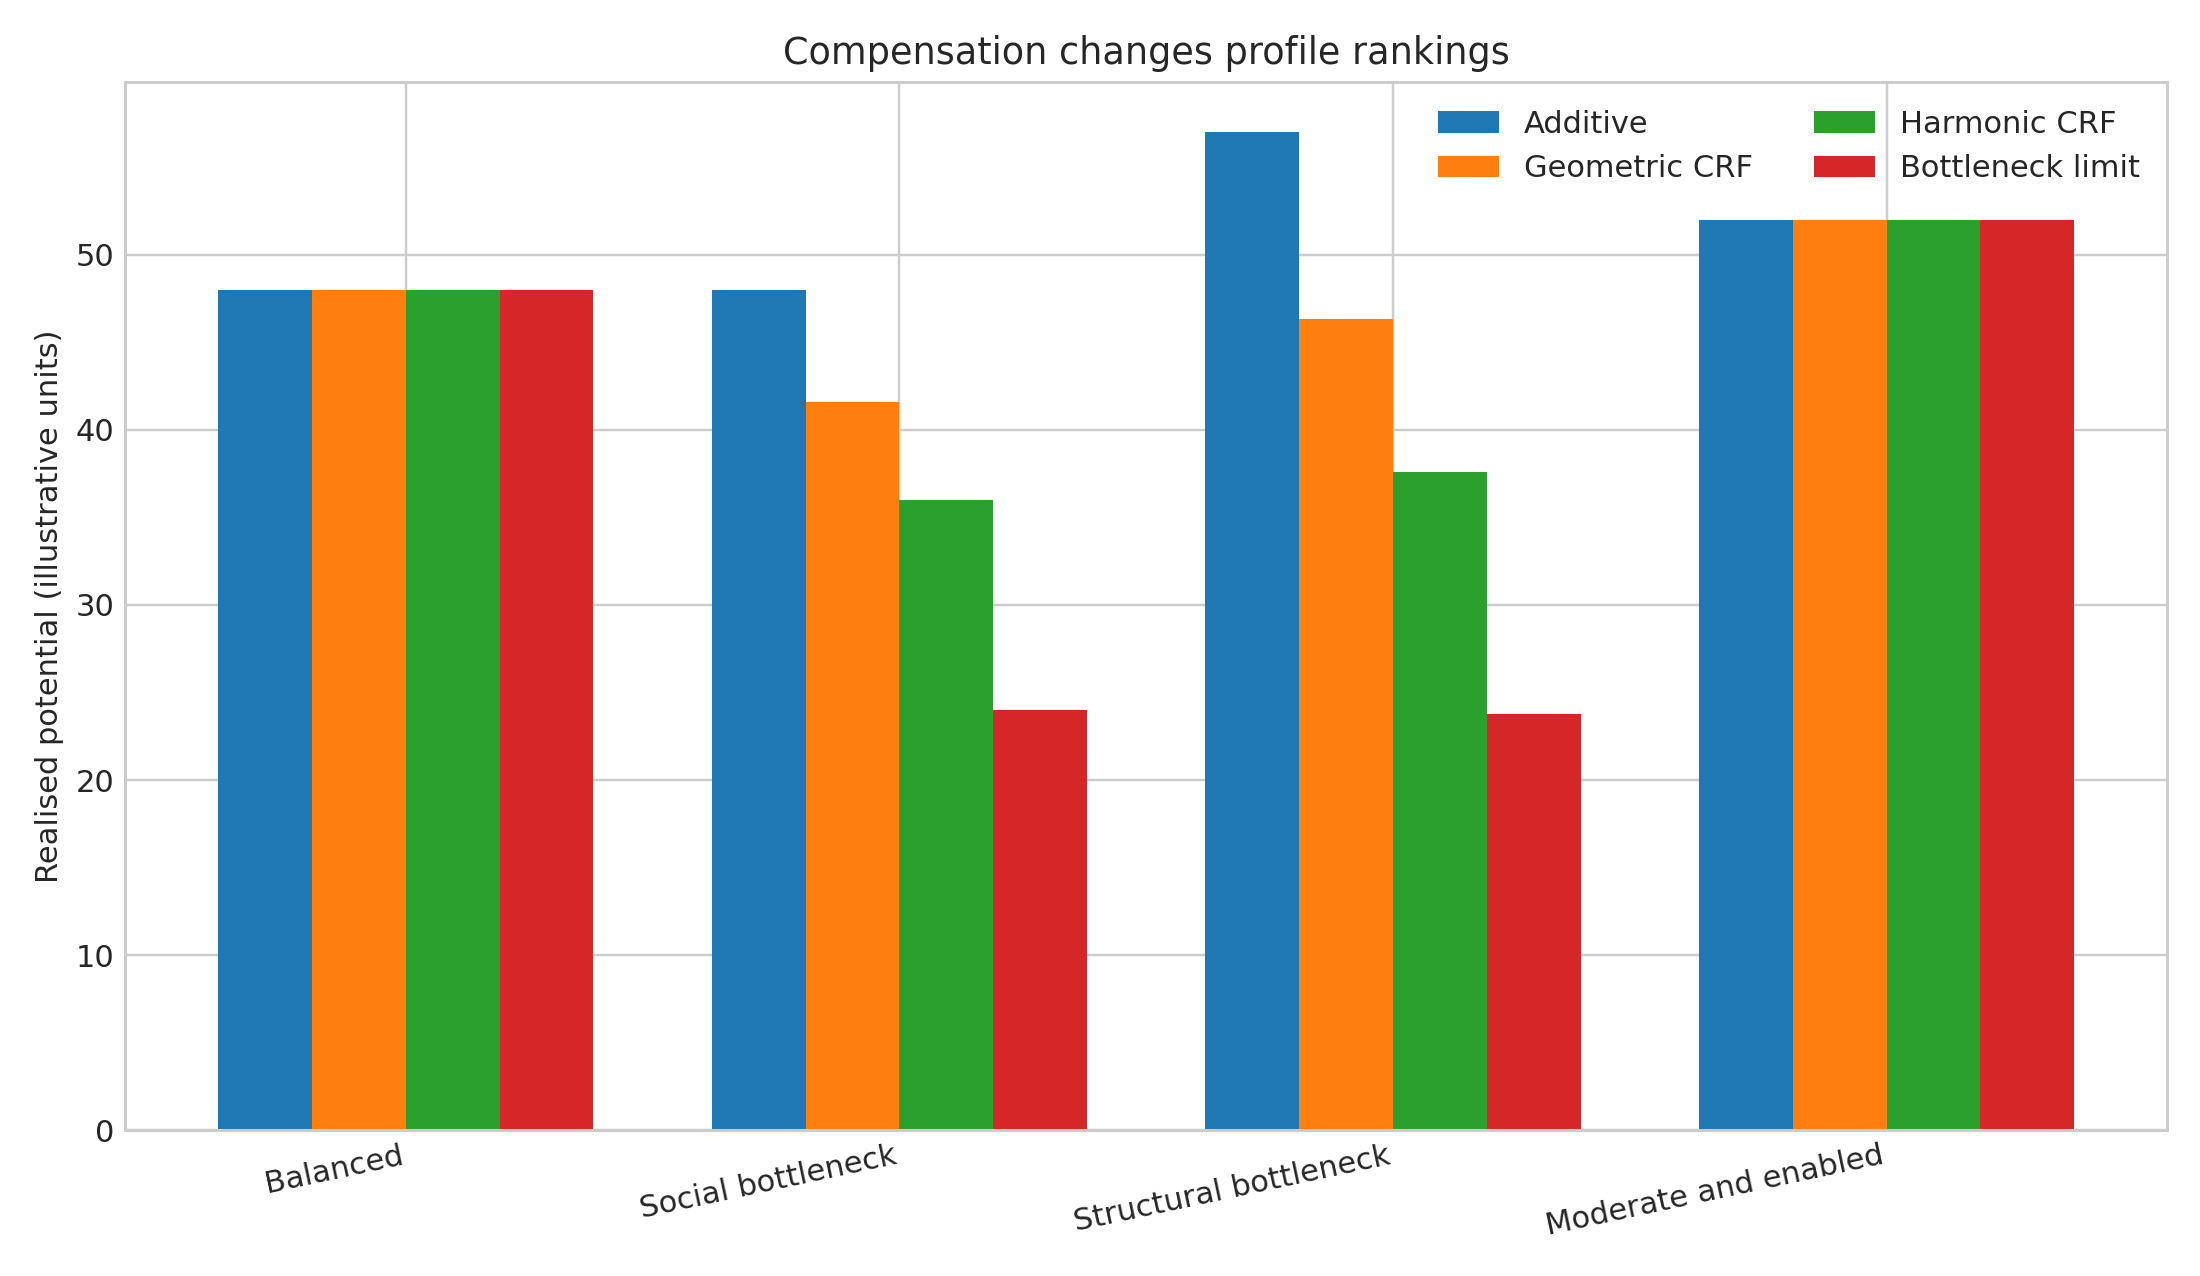
\includegraphics[width=0.9\textwidth]{Figures/crf_profile_comparison.png}
\caption{Illustrative profile rankings under compensatory and non-compensatory
aggregators. Profiles with equal average contextual resources can separate under
the CRF when one enabling domain is a bottleneck. Values are simulated.}
\label{fig:crf_profile_comparison}
\end{figure}

\begin{figure}[H]
\centering
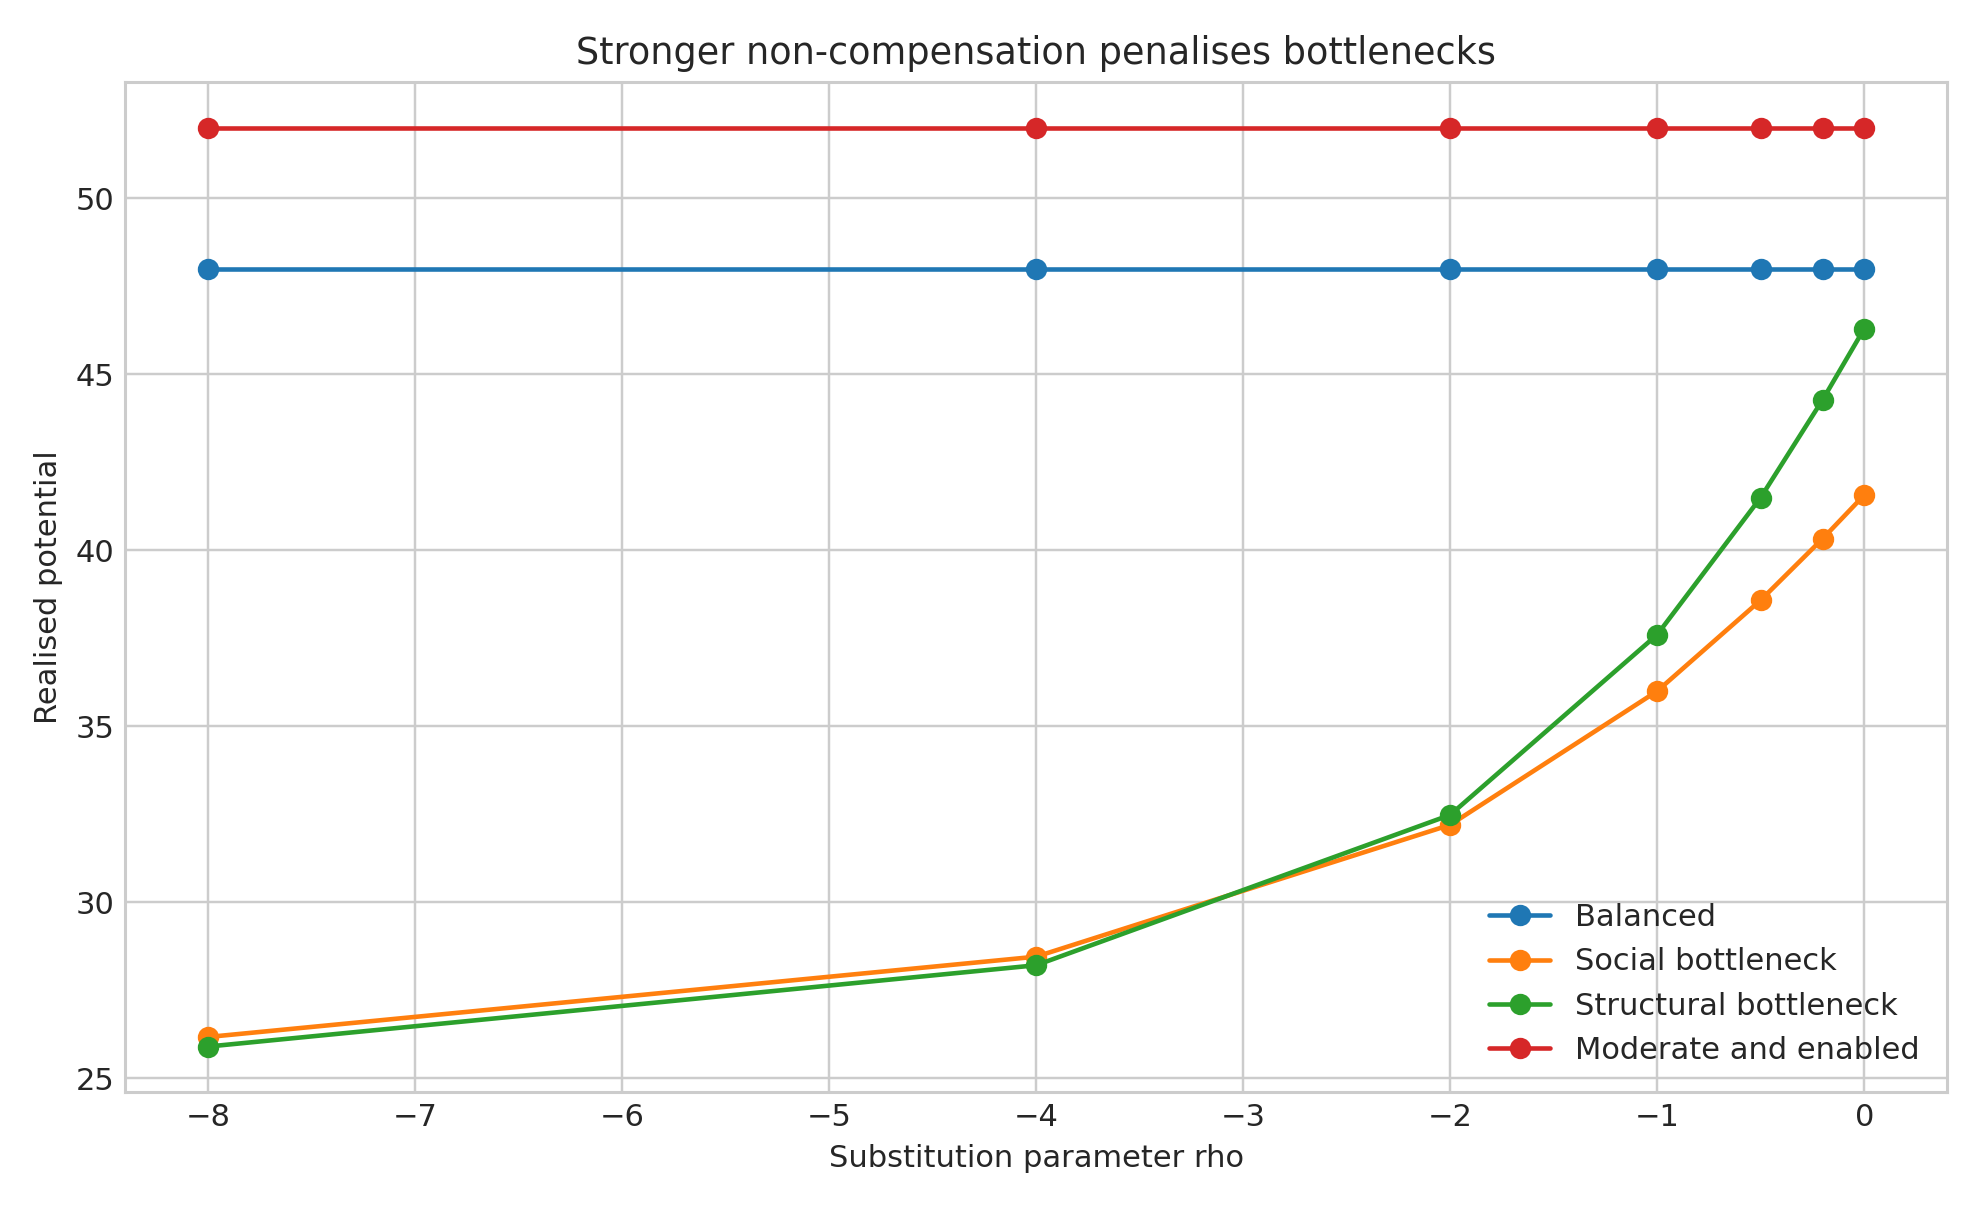
\includegraphics[width=0.9\textwidth]{Figures/crf_rho_sensitivity.png}
\caption{Sensitivity of realised potential to the substitution parameter $\rho$.
More negative values impose a stronger bottleneck penalty. Values are simulated.}
\label{fig:crf_rho_sensitivity}
\end{figure}

\begin{figure}[H]
\centering
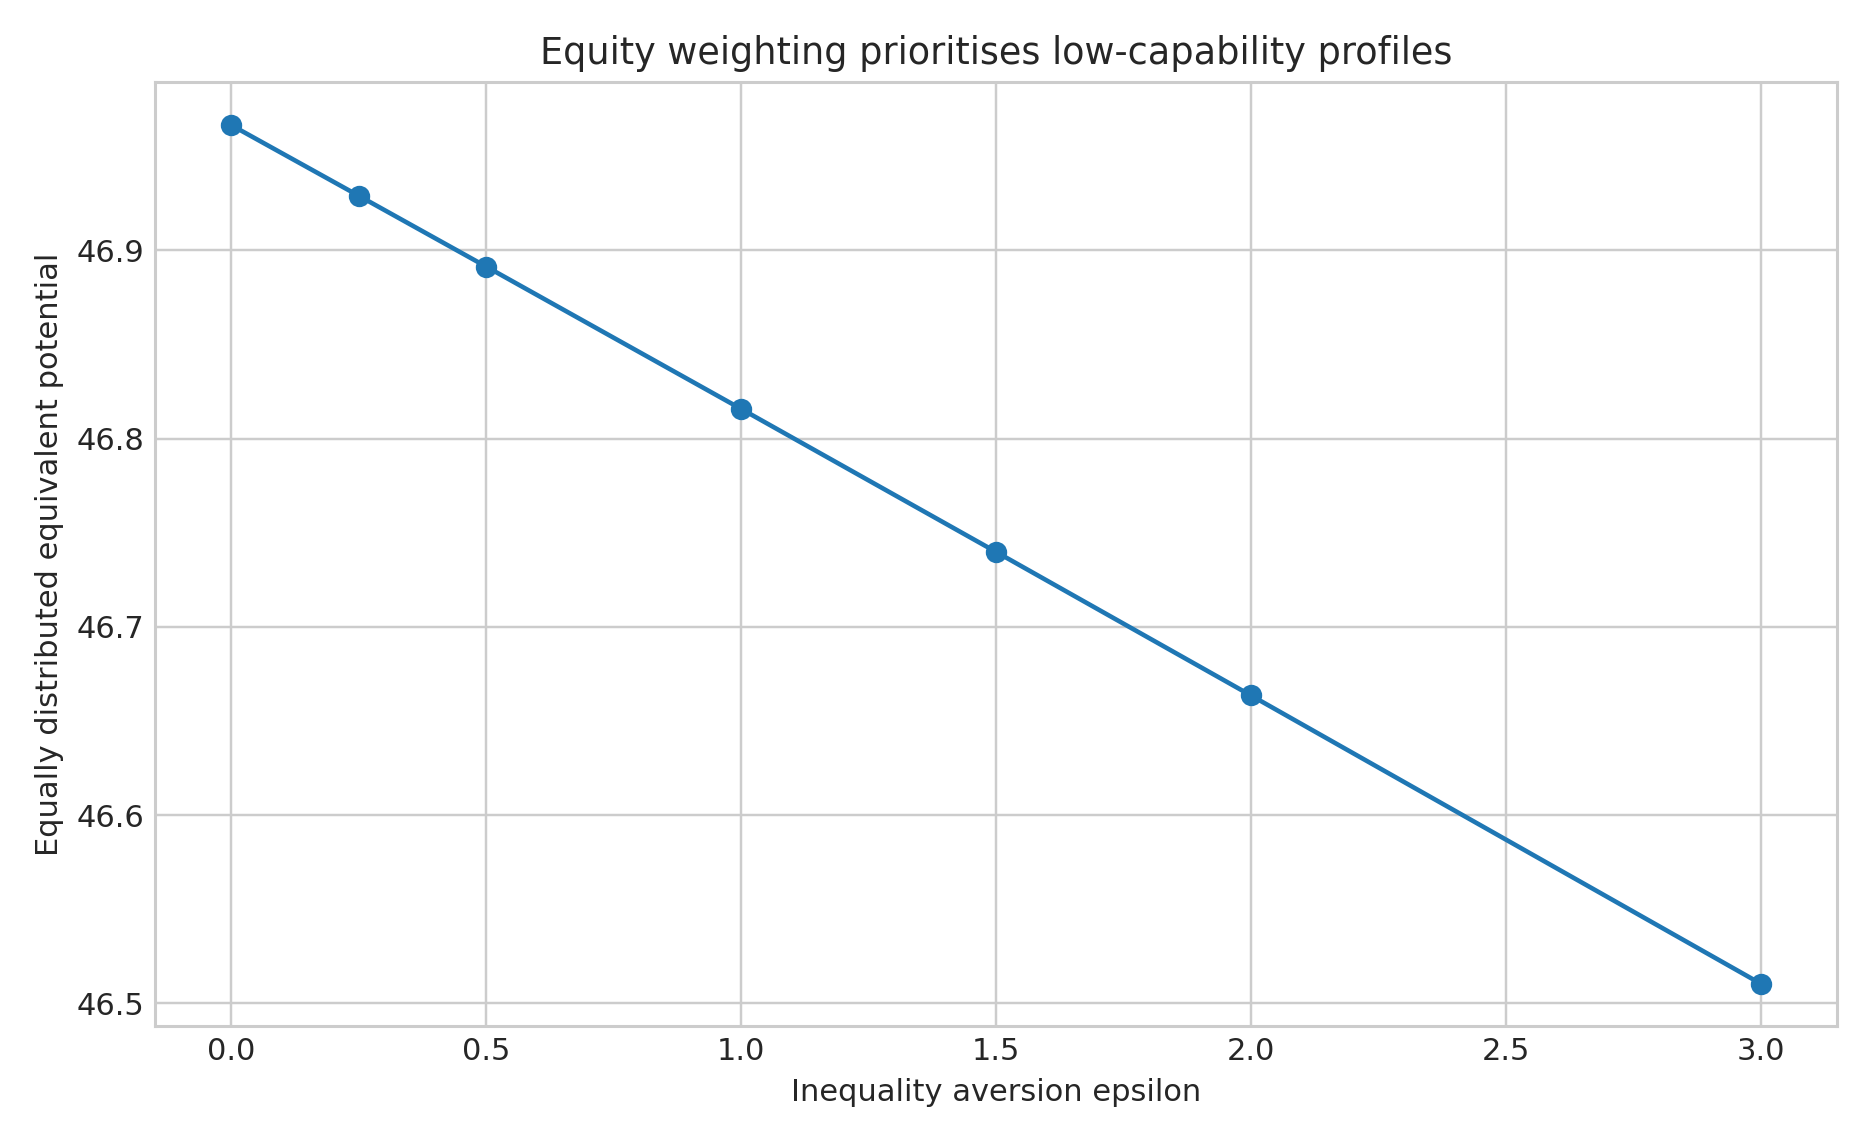
\includegraphics[width=0.9\textwidth]{Figures/crf_equity_aversion.png}
\caption{Equally distributed equivalent potential as inequality aversion
$\varepsilon$ increases. Declines indicate that low-capability profiles receive
greater normative weight. Values are simulated.}
\label{fig:crf_equity_aversion}
\end{figure}

The generated CSV files preserve every plotted value and include model-implied
marginal gains for biomedical, social, and burden-reducing interventions. These
gradients illustrate how aggregation can change priorities; they are not causal
treatment effects.

\section{Falsification and Empirical Comparison}
\label{sec:E-falsification}
The mathematical contribution is supported only if the following pre-specified
tests succeed:
\begin{enumerate}
 \item domain orientations and boundary behaviour are empirically plausible;
 \item CRF scores are stable under defensible normalisation choices;
 \item the non-compensatory model is compared with an additive composite, the SEM
 factor score, and less restrictive $\rho>0$ sensitivity models;
 \item paired bootstrap \citep{efron_tibshirani_1993,steyerberg_2019} estimates compare calibration, discrimination, and net
 benefit without tuning $\alpha$ or $\rho$ to the evaluation outcomes;
 \item subgroup analyses assess whether the model reduces or amplifies systematic
 error; and
 \item external validation evaluates transportability of both levels and gradients.
\end{enumerate}
Failure of these tests rejects or narrows the CRF; it does not invalidate the
separate latent measurement model.

\subsection{Head-to-head empirical protocol}
The empirical comparison uses the same analytic sample, imputations, resamples,
outcomes, and evaluation horizons for every representation:
\begin{enumerate}
 \item age-and-sex baseline;
 \item conventional comparator set (frailty, comorbidity, function, and QALY
 proxy);
 \item additive domain composite;
 \item primary SEM factor score;
 \item geometric CRF; and
 \item CRF sensitivity specifications for pre-declared $\rho$ values.
\end{enumerate}
All normalisation bounds, $\alpha$, $\rho$, and indicator directions are frozen
without reference to mortality or hospitalisation. Within each paired bootstrap
replicate the full measurement and prognostic pipeline is repeated. Reported
contrasts include calibration intercept and slope, time-specific Brier score \citep{brier_1950},
Harrell and Uno concordance \citep{uno_2011}, time-dependent AUC, and net benefit. Subgroup
calibration and error are reported across pre-specified equity strata.

\subsection{Success and rejection criteria}
The mathematical model is not declared useful merely because a CRF coefficient is
statistically significant. A strong mathematical--empirical contribution requires:
\begin{enumerate}
 \item rejection of the claim that the CRF is numerically redundant with the
 additive composite, demonstrated by meaningful profile or ranking differences;
 \item calibration and overall prediction error no worse than the additive and SEM
 alternatives, with paired uncertainty;
 \item either improved net benefit \citep{vickers_elkin_2006} over a clinically defensible threshold range or
 demonstrably clearer detection of structural bottlenecks;
 \item no material worsening of subgroup calibration or error; and
 \item qualitatively stable conclusions across reasonable normalisation bounds and
 pre-specified $\rho$ values.
\end{enumerate}
If these conditions fail, the central empirical claim for the CRF is narrowed to a
theoretical model, and the outcome-independent SEM score is retained as the
measurement backbone. If they hold internally but not externally, the claim is
restricted to the developmental population.

\subsection{Explicit rejection criteria}
The construct and its realisation model are rejected or narrowed if any pre-specified
condition holds under outcome-blind evaluation.
\begin{enumerate}\setlength{\itemsep}{2pt}
\item \textbf{Measurement collapse.} The three domains fail discriminant validity
($\mathrm{HTMT}>0.85$, or factor correlations above $0.90$), forcing a single factor.
\item \textbf{Determinacy failure.} The second-order factor-score determinacy \citep{grice_2001} falls
below $0.80$, so a person-level scalar cannot be reliably estimated.
\item \textbf{Prognostic non-inferiority deficit.} In optimism-corrected bootstrap
comparisons the full model fails to improve discrimination ($\Delta C\le 0$) or
prediction error over a parsimonious frailty or comorbidity index.
\item \textbf{Non-compensatory rejection.} The geometric CRF shows a worse calibration
slope, $|1-b_{\text{geom}}|>|1-b_{\text{add}}|$, or lower net benefit than an additive
composite.
\item \textbf{Invariance breakdown.} Scalar invariance \citep{putnick_bornstein_2016} fails across major groups and
partial invariance cannot restore fit, so group differences reflect measurement bias.
\end{enumerate}
If criterion~1 or~2 holds, the scalar metric is abandoned for the unaggregated
profile $(P,S,R)$. If criterion~4 holds, the non-compensatory hypothesis is refuted
and compensatory additive modelling is restored. Declaring these before the outcome
analysis is what makes the framework interrogable.

\section{Summary}
The CRF supplies the thesis with a dimensionally coherent and falsifiable
mathematical object. Its distinctive contribution is not the geometric mean alone,
but the combined axioms, non-compensatory interpretation, complementarity proof,
exact equity-gap decomposition, causal caveat, and pre-specified comparison with
the outcome-independent SEM metric.
